\section{平行移动}
\label{sec:riem-parallel-transport}

联络回答“沿曲线走时向量变了多少”，反过来就能规定“沿曲线走时向量保持不变”的含义：协变导数处处为零。从起点的一个切向量出发，沿曲线一路保持不变，到达终点时得到终点处的一个切向量。这就给出了比较不同点处切向量的方式，只是比较的结果要依赖所走的路线。

\paragraph{平行向量场}
设$\gamma:[a,b]\to M$是分段光滑曲线，$V$是沿$\gamma$的向量场。若在每个光滑段上$DV/\mathrm dt=0$，并且$V$在分点处连续，就称$V$沿$\gamma$\emph{平行}。由式~\eqref{eq:riem-covariant-derivative-along-curve}，在一张坐标图内这个条件是关于分量$V_1,\ldots,V_n$的方程组
\begin{equation}
\dot V_k(t)=-\sum_{i,j}\Gamma^k_{i,j}\bigl(x(t)\bigr)\,\dot x_i(t)\,V_j(t),\qquad k=1,\ldots,n .
\label{eq:riem-parallel-equation}
\end{equation}
曲线$x(t)$已经给定，右端的系数$a_{k,j}(t)=-\sum_i\Gamma^k_{i,j}(x(t))\dot x_i(t)$只是$t$的连续函数，所以这是一个线性常微分方程组$\dot{\bm V}=\bm A(t)\bm V$。

\paragraph{所需的常微分方程结论}
线性方程有一个比一般非线性方程更强的性质：解不会在区间内部“跑掉”。对线性方程，$\lVert\bm V\rVert$的增长速度至多与$\lVert\bm V\rVert$本身成比例，所以解至多按指数增长，不会在有限时间内趋于无穷。下面陈述所用的结论。

\begin{theorem}[线性常微分方程的整体存在唯一性]
\label{thm:riem-linear-ode}
设$\bm A:[a,b]\to\mathbb R^{n\times n}$连续，$t_0\in[a,b]$，$\bm V_0\in\mathbb R^n$。则初值问题$\dot{\bm V}(t)=\bm A(t)\bm V(t)$、$\bm V(t_0)=\bm V_0$在整个$[a,b]$上存在唯一的$C^1$解，并且解在每个时刻$t$的值线性地依赖于$\bm V_0$。
\end{theorem}

证明需要一般的存在性与延拓理论，读者可查阅\BookChapterRef{chap:ode-existence-continuation}{卷六第3章“解的存在性”}。线性依赖一半来自唯一性：若$\bm V$与$\bm W$分别是初值$\bm V_0$与$\bm W_0$的解，则$c\bm V+\bm W$满足同一方程且初值为$c\bm V_0+\bm W_0$，由唯一性它就是后者的解。

\paragraph{平行移动的定义}
把定理~\ref{thm:riem-linear-ode}用于方程~\eqref{eq:riem-parallel-equation}，需要先处理曲线跨越多张坐标图的情形。由于$\gamma([a,b])$紧，可以把$[a,b]$分成有限段，使每段落在一张图内并且光滑。在第一段上求解，以终值作为下一段的初值，依次进行。重叠处的两种坐标描述的是同一个方程$DV/\mathrm dt=0$，唯一性保证结果与分段方式无关。

\begin{definition}[平行移动]
\label{def:riem-parallel-transport}
设$\gamma:[a,b]\to M$分段光滑，$p=\gamma(a)$，$q=\gamma(b)$。对$\bm v\in T_pM$，记$V$为沿$\gamma$满足$V(a)=\bm v$的唯一平行向量场，定义
\begin{equation}
P_\gamma:T_pM\to T_qM,\qquad P_\gamma(\bm v)=V(b).
\label{eq:riem-parallel-transport}
\end{equation}
$P_\gamma$称为沿$\gamma$的\term{平行移动}（parallel transport）。
\end{definition}

由定理~\ref{thm:riem-linear-ode}，$P_\gamma$是线性映射。把曲线反向得到$\bar\gamma(t)=\gamma(a+b-t)$，沿$\bar\gamma$平行的场恰是沿$\gamma$平行的场倒过来读，所以$P_{\bar\gamma}\circ P_\gamma=\operatorname{id}$，$P_\gamma$是线性同构。两条曲线首尾相接时，平行移动相应复合。这里只要求曲线分段光滑，不需要流形具有任何整体性质。

\begin{theorem}[平行移动保持内积]
\label{thm:riem-transport-isometry}
设$\nabla$是$(M,g)$的Levi-Civita联络。则对任意分段光滑曲线$\gamma$及$\bm u,\bm v\in T_{\gamma(a)}M$，有
\begin{equation}
g\bigl(P_\gamma\bm u,P_\gamma\bm v\bigr)=g(\bm u,\bm v).
\label{eq:riem-transport-isometry}
\end{equation}
\end{theorem}

\begin{proof}
设$U,V$是沿$\gamma$分别以$\bm u,\bm v$为初值的平行向量场。先证沿曲线的乘积法则。在坐标中写$g(U,V)=\sum_{i,j}g_{i,j}(x(t))U_iV_j$，对$t$求导，其中度量系数的导数由式~\eqref{eq:riem-compatible-coordinates}写成
\[
\frac{\mathrm d}{\mathrm dt}g_{i,j}(x(t))=\sum_k\dot x_k\bigl(\Gamma_{k,i;j}+\Gamma_{k,j;i}\bigr).
\]

把这一项与$U_i,V_j$的导数合并，得到
\[
\frac{\mathrm d}{\mathrm dt}g(U,V)=g\Bigl(\frac{DU}{\mathrm dt},V\Bigr)+g\Bigl(U,\frac{DV}{\mathrm dt}\Bigr).
\]

$U,V$平行，右端为零。于是内积在各光滑段上为常数，又在分点处连续，所以在整个$[a,b]$上不变。
\end{proof}

于是平行移动保持长度和夹角。这个结论用到了度量相容；对一般联络，平行移动只是线性同构，可以拉长或压缩向量。

\paragraph{平行移动依赖路径}
在欧氏空间中取通常的联络，直角坐标中系数为零，方程~\eqref{eq:riem-parallel-equation}给出分量不变：沿任何曲线搬运，向量都保持原样，终点处的结果与路径无关。弯曲的空间不再如此。

\begin{example}[球面上沿三段大圆弧的搬运]
\label{ex:riem-sphere-transport}
在单位球面$S^2$上取北极$N=(0,0,1)$、$A=(1,0,0)$、$B=(0,1,0)$，沿四分之一大圆弧$N\to A\to B\to N$搬运$\bm v=\bm e_1\in T_NS^2$。用投影公式~\eqref{eq:riem-projection-connection}，沿曲线平行的条件是环境导数$\dot V$与球面垂直，即平行于位置向量。三段都用$t\in[0,\pi/2]$参数化：
\begin{center}
\begin{tabular}{@{}lll@{}}
\toprule
路段 & 曲线$\gamma(t)$ & 向量$V(t)$\\
\midrule
$N\to A$ & $(\sin t,0,\cos t)$ & $(\cos t,0,-\sin t)$\\
$A\to B$ & $(\cos t,\sin t,0)$ & $(0,0,-1)$\\
$B\to N$ & $(0,\cos t,\sin t)$ & $(0,\sin t,-\cos t)$\\
\bottomrule
\end{tabular}
\end{center}

逐段核对。三段都有$\langle\gamma,V\rangle=0$，所以$V$切于球面。三段的导数依次为
\[
\dot V=-\gamma,\qquad\dot V=\bm 0,\qquad\dot V=\gamma,
\]
都平行于位置向量，投影为零。

两个接点$A,B$处的向量都是$(0,0,-1)$，衔接连续。回到$N$时$t=\pi/2$，
\[
V=(0,1,0)=\bm e_2 .
\]
\end{example}

图~\ref{fig:riem-octant-transport}画出了这段搬运。从$\bm e_1$出发绕一圈回来得到$\bm e_2$，转过了$\pi/2$；若一直停在$N$，向量当然不变。所以平行移动不能只由起点和终点确定，必须指定路径。

\begin{BookInlineFigure}
  \centering
  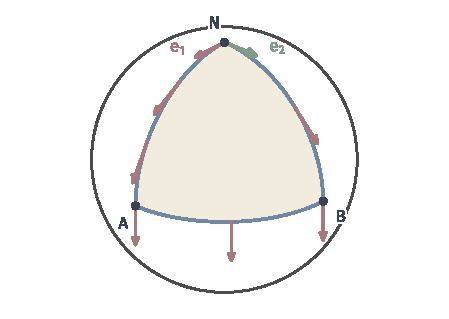
\includegraphics[width=76mm]{figures/04-spaces-measures-and-geometry/04-manifolds/matplotlib/riem-octant-transport/figure.pdf}
  \caption{球面八分之一三角形$N\to A\to B\to N$（黄色）上的平行移动。红箭头是例~\ref{ex:riem-sphere-transport}给出的向量$V(t)$，它沿每段大圆保持与路线的固定夹角；回到$N$时变为绿箭头$\bm e_2$，与初始的$\bm e_1$成直角。}
  \label{fig:riem-octant-transport}
\end{BookInlineFigure}

转角恰好等于这块球面三角形的面积$4\pi/8=\pi/2$。这个巧合在下面的例子中再次出现，第~\ref{sec:riem-curvature}节将用曲率解释。

\begin{example}[沿纬线的平行移动]
\label{ex:riem-latitude-transport}
沿过$p=(0,\tfrac35,\tfrac45)$的纬线搬运一个切向量。记$\theta_0$为$p$的极角，
\[
\sin\theta_0=\tfrac35,\qquad\cos\theta_0=\tfrac45 .
\]
路线取$(\theta,\phi)=(\theta_0,\tfrac\pi2+t)$，$t\in[0,2\pi]$。此时$\dot\theta=0$、$\dot\phi=1$，方程~\eqref{eq:riem-parallel-equation}化为
\[
\dot V_\theta=\sin\theta_0\cos\theta_0\,V_\phi,\qquad\dot V_\phi=-\cot\theta_0\,V_\theta .
\]

$\partial_\phi$的长度是$\sin\theta_0$，改用单位向量的分量会更清楚。令
\[
\bm e_\theta=\partial_\theta,\qquad\bm e_\phi=\frac{\partial_\phi}{\sin\theta_0},\qquad V=a\,\bm e_\theta+b\,\bm e_\phi ,
\]
则$V_\theta=a$，$V_\phi=b/\sin\theta_0$，代入得到
\[
\dot a=\cos\theta_0\,b,\qquad\dot b=-\cos\theta_0\,a .
\]

这是匀速旋转的方程。取初值$a(0)=1$、$b(0)=0$，也就是$p$处指向南方的单位向量，解为
\[
a(t)=\cos(\tfrac45t),\qquad b(t)=-\sin(\tfrac45t).
\]

绕一圈回到$p$时$t=2\pi$，$\tfrac45t=\tfrac{8\pi}5$，于是
\[
a(2\pi)=\cos\tfrac{2\pi}5\approx0.309,\qquad b(2\pi)=\sin\tfrac{2\pi}5\approx0.951 .
\]
向量从$\bm e_\theta$朝$\bm e_\phi$方向转过了$\tfrac{2\pi}5$。北极冠的面积是$2\pi(1-\cos\theta_0)=\tfrac{2\pi}5$，转角再次等于所围面积。
\end{example}

纬线的例子还可以用一张平面图来理解。沿纬线作球面的切锥，切点处锥面与球面有相同的切平面。对沿纬线的向量场，平行的条件只是“$\dot V$垂直于切平面”，所以在球面上平行与在切锥上平行是同一个条件。切锥可以摊平成平面扇形，半径$\tan\theta_0=\tfrac34$，圆心角$2\pi\cos\theta_0=\tfrac{8\pi}5$。在摊平的扇形上，平行向量就是常向量。

图~\ref{fig:riem-latitude-transport}(b)就是这个扇形：红箭头在平面上始终平行，$p$在扇形的两条边上各出现一次。扇形的缺口恰好是$\tfrac{2\pi}5$，这正是绕一圈的转角。

\begin{BookInlineFigure}
  \centering
  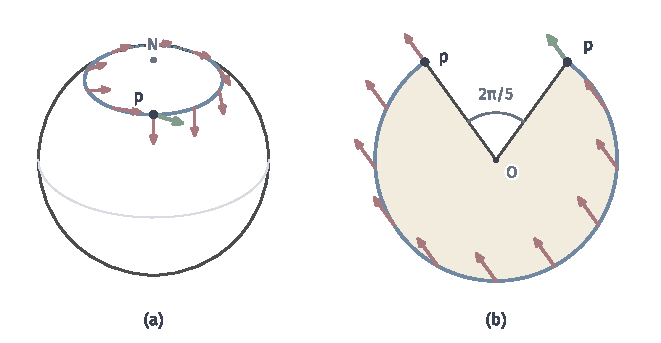
\includegraphics[width=112mm]{figures/04-spaces-measures-and-geometry/04-manifolds/matplotlib/riem-latitude-transport/figure.pdf}
  \caption{沿纬线的平行移动。(a)过$p=(0,\tfrac35,\tfrac45)$的纬线（蓝色）上，红箭头是从向南的单位向量出发平行移动的结果，绕一圈回到$p$时变为绿箭头，转过$\tfrac{2\pi}5$。(b)切锥摊平成的扇形，圆心角$\tfrac{8\pi}5$，缺口$\tfrac{2\pi}5$，纬线是外圆弧，$O$是锥顶。沿纬线的平行向量在扇形上是常向量，两条边是锥面上同一条母线。}
  \label{fig:riem-latitude-transport}
\end{BookInlineFigure}

\paragraph{与映射的微分比较}
第~\ref{chap:manifold-maps}章中，光滑映射$F:M\to N$在每点诱导线性映射$\mathrm dF_p:T_pM\to T_{F(p)}N$。平行移动$P_\gamma$也是切空间之间的线性映射，但二者的输入完全不同，表~\ref{tab:riem-transport-vs-differential}列出了对照。

\begin{BookInlineTable}
  \centering
  \begin{tabular}{lll}
    \toprule
    & 微分$\mathrm dF_p$ & 平行移动$P_\gamma$\\
    \midrule
    需要的输入 & 点映射$F$ & 曲线$\gamma$与联络\\
    是否需要度量 & 不需要 & 取Levi-Civita联络时需要\\
    依赖的范围 & $F$在$p$附近的取值 & 整条曲线\\
    \bottomrule
  \end{tabular}
  \caption{切空间之间的两种线性映射。}
  \label{tab:riem-transport-vs-differential}
\end{BookInlineTable}

在欧氏平面上取绕原点旋转角$\alpha$的映射$F$，则$\mathrm dF_p\bm v=\bm R_\alpha\bm v$，向量随之转过$\alpha$。而沿任何从$p$到$F(p)$的曲线作平行移动，得到的都是$\bm v$本身。两者都把$T_pM$映到$T_{F(p)}M$，结果却相差一个旋转。后面讨论等距映射与Lie群作用时，需要分清向量是“被映射带过去”还是“沿路径搬过去”的。
